\begin{appendices}
    \chapter{Position des stop}
    \begin{figure}[ht]
        \centering
        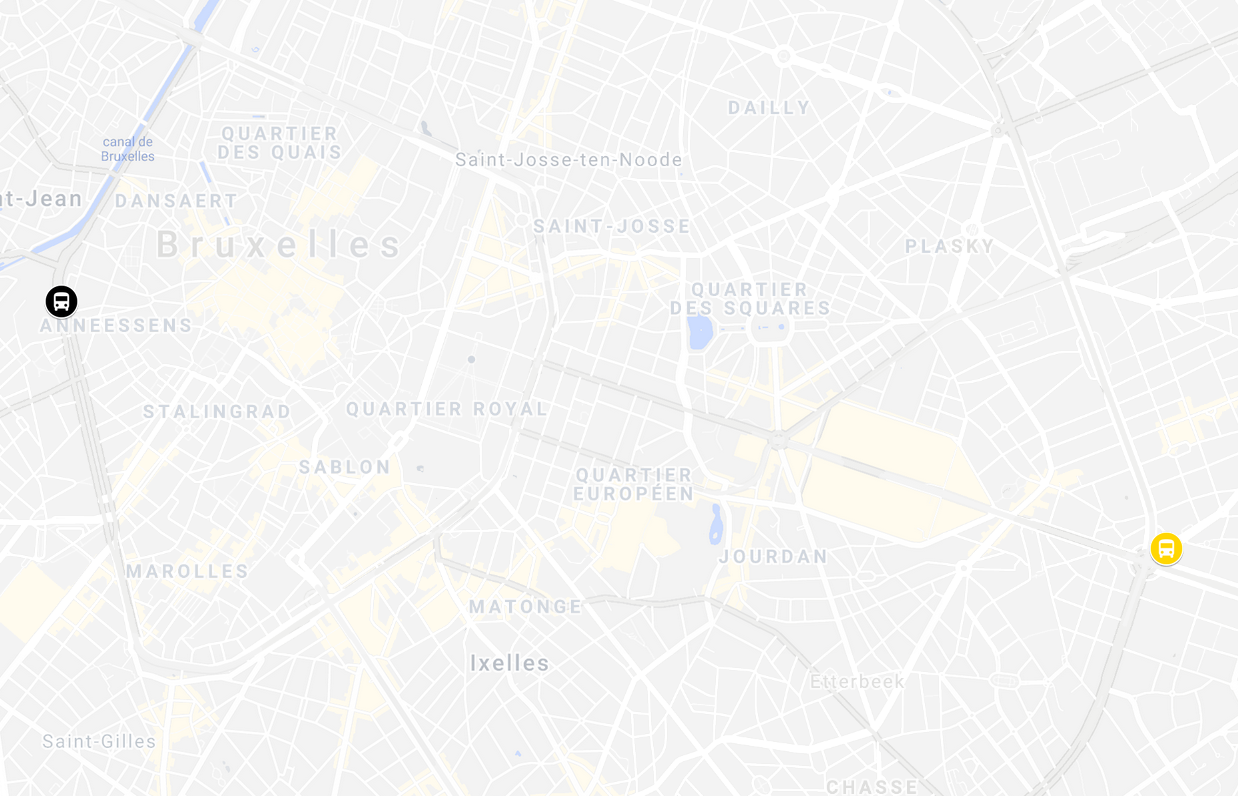
\includegraphics[width=0.7\textwidth]{images/stop_pos_1.png}
        \caption{Position des stop numéro 0089 et 6608G en jaune et noir respectivement.}
        \label{appendix:stop_pos_1}
    \end{figure}

    \begin{figure}[ht]
        \centering
        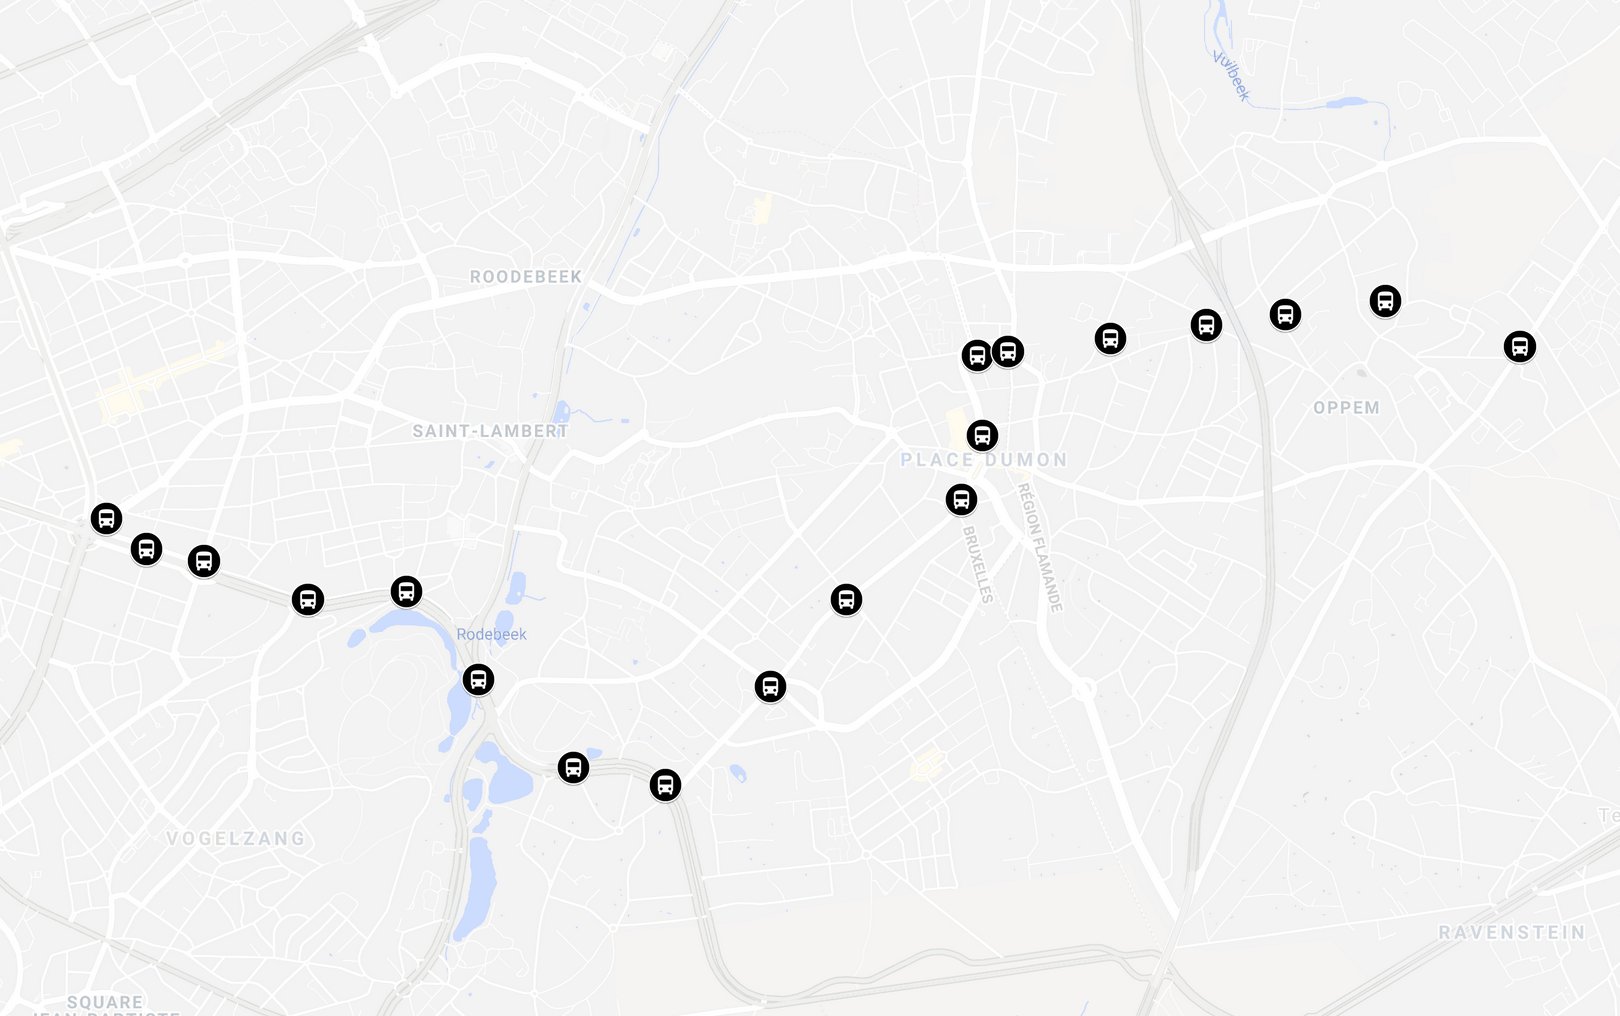
\includegraphics[width=0.7\textwidth]{images/stop_pos_2.png}
        \caption{Position des stop présents sur la ligne 39}
        \label{appendix:stop_pos_2}
    \end{figure}

    \chapter{Première visualisation des données}
    \begin{figure}[ht]
        \centering
        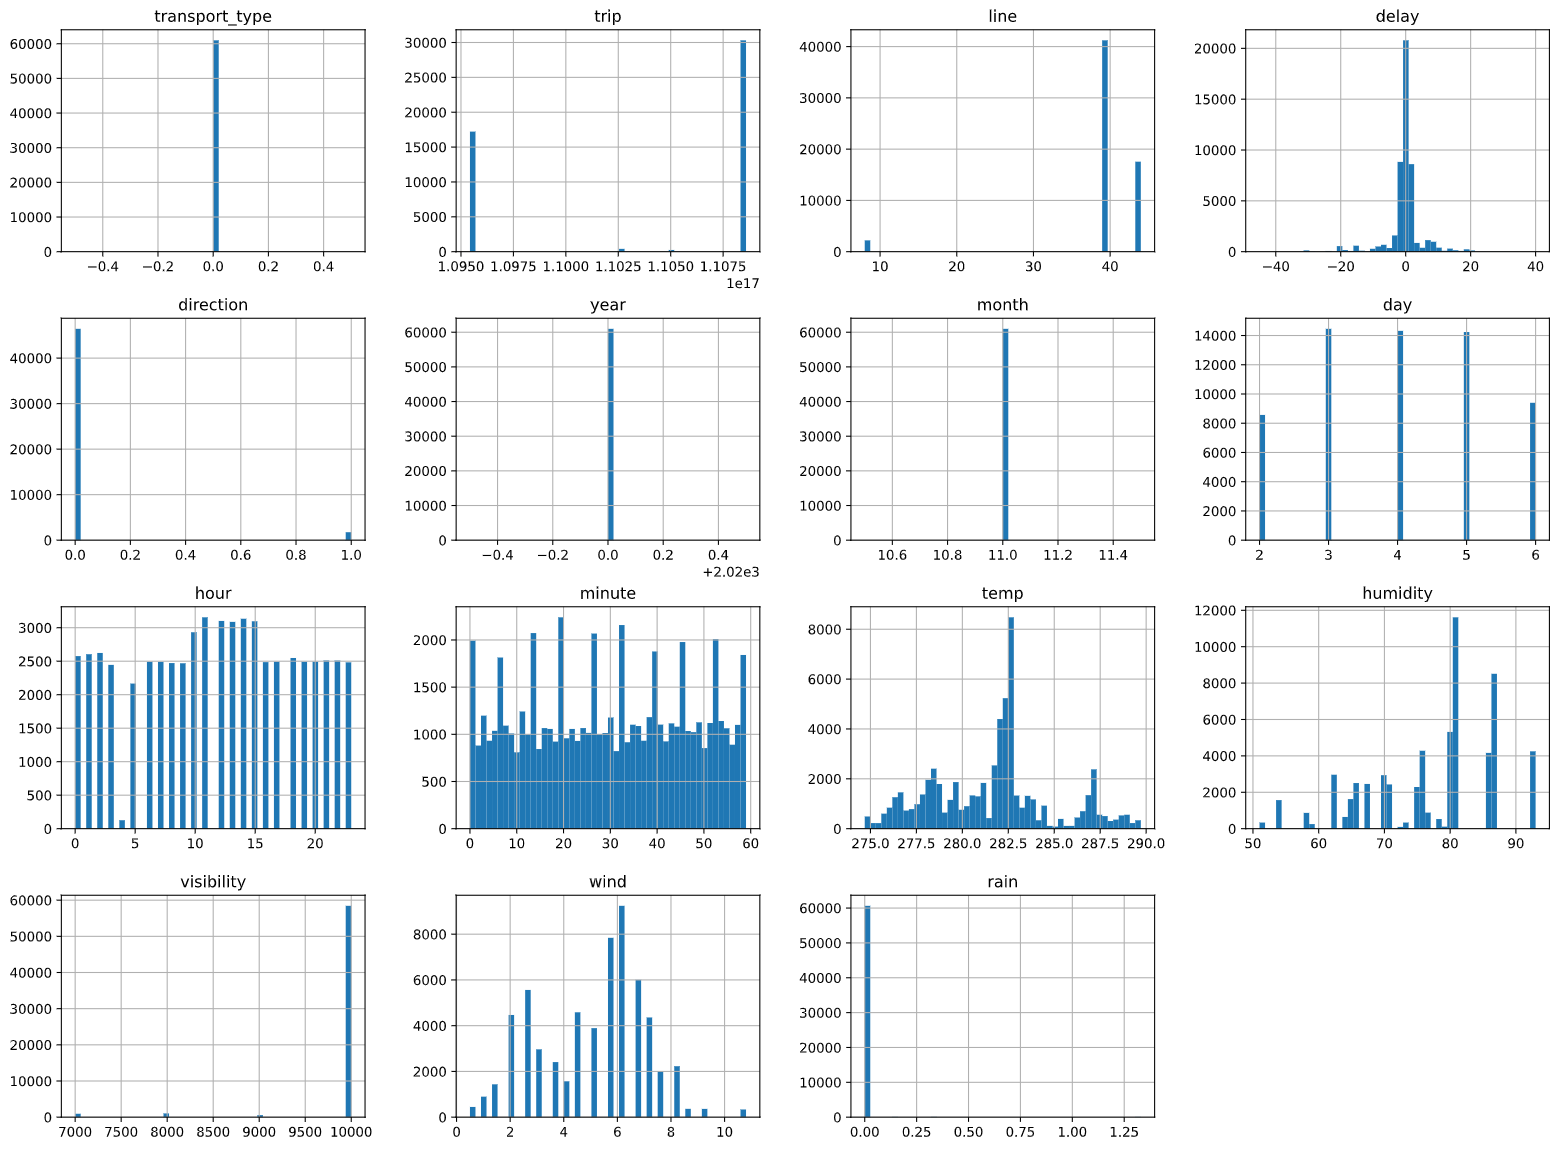
\includegraphics[width=0.7\textwidth]{images/plots.png}
        \caption{Plot des features par nombre d'occurrences}
        \label{appendix:plots}
    \end{figure}

    \begin{figure}[ht]
        \centering
        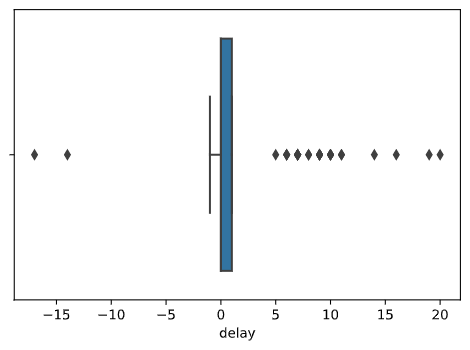
\includegraphics[width=0.7\textwidth]{images/boxplot.png}
        \caption{Boxplot des délais du 19 septembre sur la ligne 39 au stop 0089}
        \label{appendix:boxplot}
    \end{figure}

    \begin{figure}[ht]
        \centering
        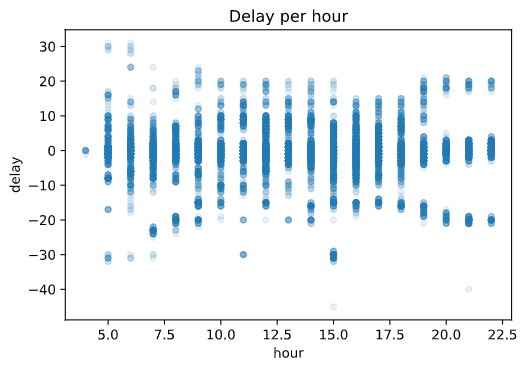
\includegraphics[width=0.7\textwidth]{images/delay_per_hour.png}
        \caption{Délais par heure pour tout le dataset}
        \label{appendix:delay_per_hour}
    \end{figure}

    \begin{figure}[ht]
        \centering
        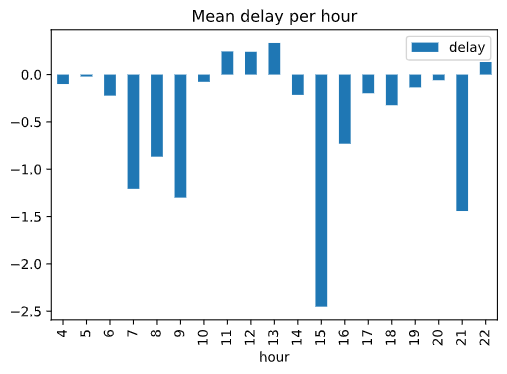
\includegraphics[width=0.7\textwidth]{images/mean_delay_per_hour.png}
        \caption{Délai moyen par heure pour tout le dataset}
        \label{appendix:mean_delay_per_hour}
    \end{figure}

    \begin{figure}[ht]
        \centering
        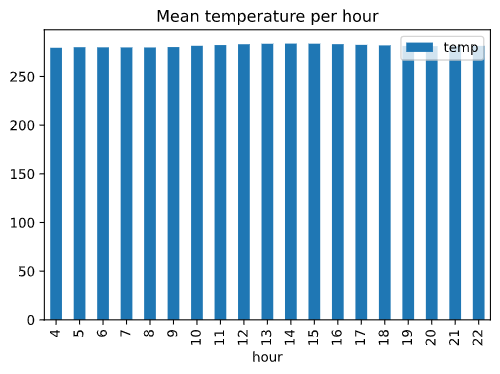
\includegraphics[width=0.7\textwidth]{images/mean_temp_per_hour.png}
        \caption{Température moyenne par heure pour tout le dataset}
        \label{appendix:mean_temp_per_hour}
    \end{figure}

    \chapter{Recherche de corrélation}
    \begin{figure}[ht]
        \centering
        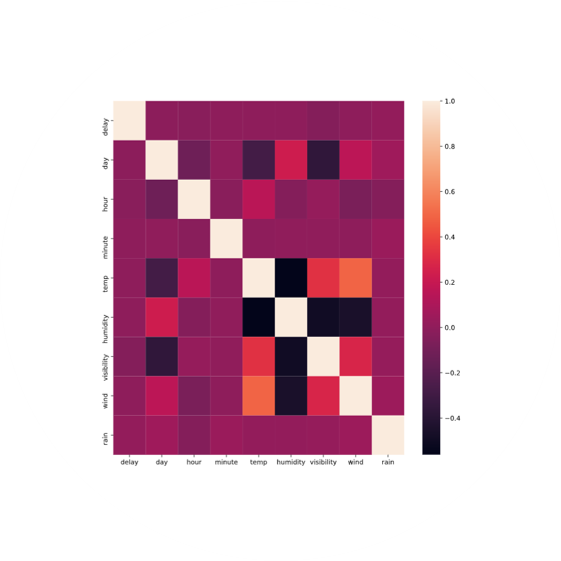
\includegraphics[width=0.7\textwidth]{images/corr_mat.png}
        \caption{Matrice de corrélation linéaire entre les différentes \textit{features}}
        \label{appendix:corr_mat}
    \end{figure}

    \begin{figure}[ht]
        \centering
        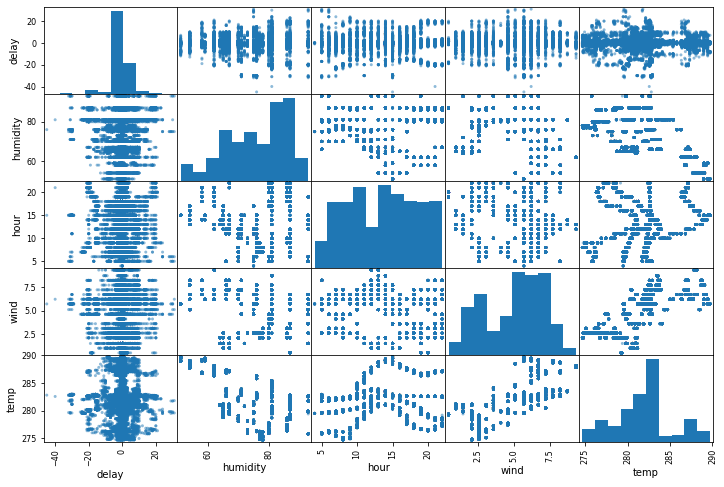
\includegraphics[width=0.7\textwidth]{images/scatter_matrix.png}
        \caption{Plot de chaque \textit{features} par rapport à chacune des autres}
        \label{appendix:scatter_matrix}
    \end{figure}

    \begin{figure}[ht]
        \centering
        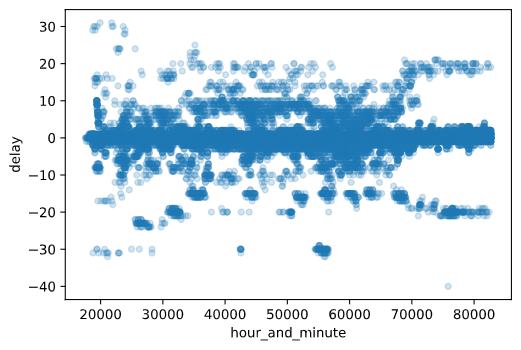
\includegraphics[width=0.7\textwidth]{images/delay_per_hour_and_minute.png}
        \caption{Délais par heure et minute pour tout le dataset}
        \label{appendix:delay_per_hour_and_minute}
    \end{figure}

    \chapter{Regression}
    \begin{table}[ht]
    \begin{tabular}{l|l|l}
        \textbf{Valeur réelle}&\textbf{Prédiction}&\textbf{Différence} \\
        \hline
        -1.0&1.02270508&-2,023 \\
        \hline
        -1.0&-1.04394531&0,044 \\
        \hline
        0.0&-1.015625&-1.016 \\
        \hline
        -1.0&0.03173828&-1,032 \\
        \hline
        -18.0&0.48291016&-18,483 \\
    \end{tabular}
    \caption{Échantillon de prédiction du modèle de régression linéaire}
    \label{appendix:linearReg}
    \end{table}

    \chapter{Classification}
    \begin{figure}[ht]
        \centering
        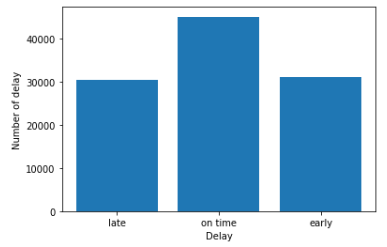
\includegraphics[width=0.7\textwidth]{images/3.png}
        \caption{Division des délais en 3 catégories}
        \label{appendix:3}
    \end{figure}

    \begin{figure}[ht]
        \centering
        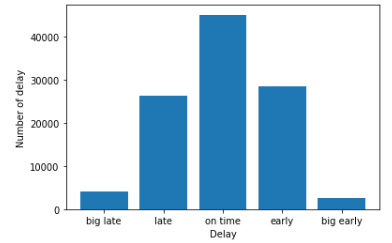
\includegraphics[width=0.7\textwidth]{images/5.png}
        \caption{Division des délais en 5 catégories}
        \label{appendix:5}
    \end{figure}

    \chapter{Conclusion}
    \begin{figure}[ht]
        \centering
        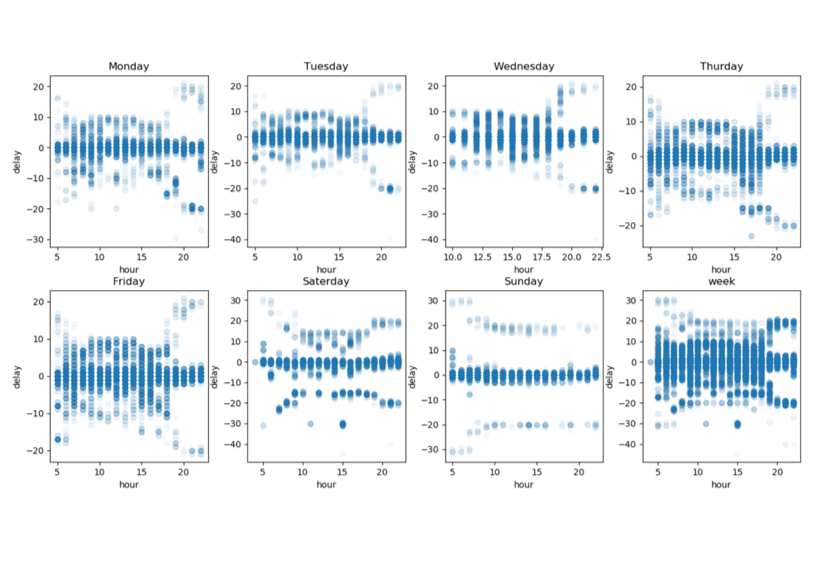
\includegraphics[width=0.7\textwidth]{images/delay_day.png}
        \caption{Le retard en fonction de l'heure par jour}
        \label{appendix:delay_day}
    \end{figure}

    \begin{figure}[ht]
        \centering
        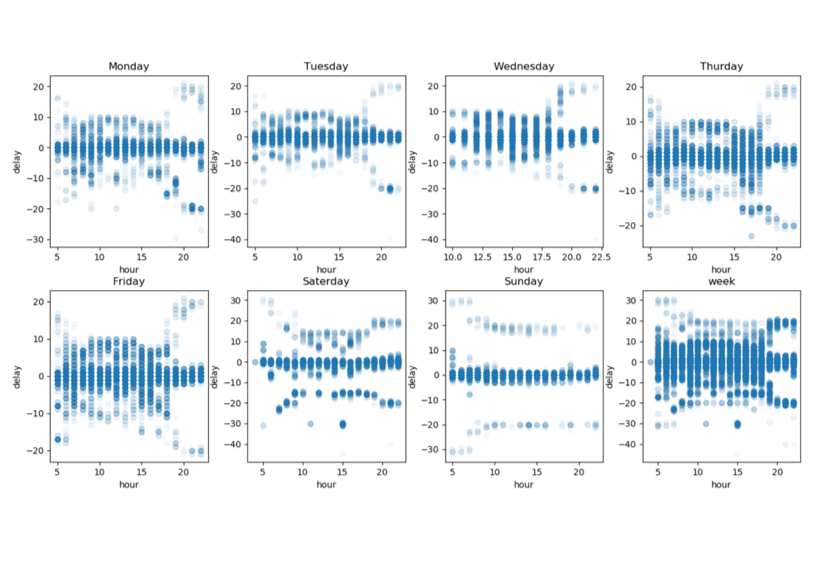
\includegraphics[width=0.7\textwidth]{images/delay_day.png}
        \caption{Le retard en fonction de l'heure par jour}
        \label{appendix:delay_day}
    \end{figure}

    \begin{figure}[ht]
        \centering
        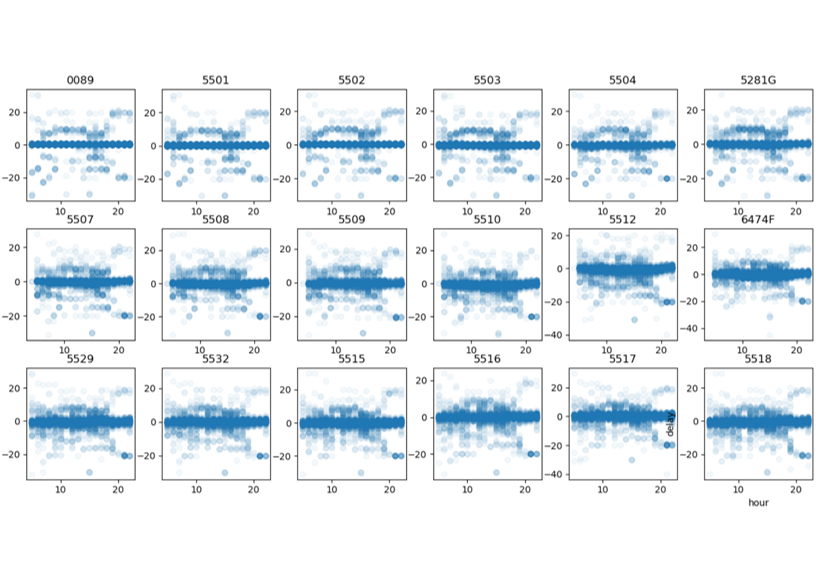
\includegraphics[width=0.7\textwidth]{images/delay_stop.png}
        \caption{Le retard en fonction de l'heure par stop}
        \label{appendix:delay_stop}
    \end{figure}

    \chapter{Bonus}
    \begin{figure}[ht]
        \centering
        
\includegraphics[width=0.7\textwidth]{images/bonus.png}
        \caption{Bonus}
        \label{appendix:bonus}
    \end{figure}

\end{appendices}